\documentclass[tikz,dvipsnames]{standalone}

\begin{document}

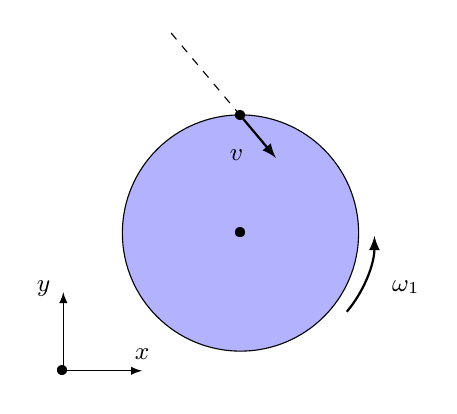
\begin{tikzpicture}

    \draw[fill=blue!30] (0,0) circle (1.5);
    \node at (0,0) {\textbullet};
    \draw[-latex,thick] (1.35,-1) arc (-40:0:1.5) node [label={[shift={(0.4,-1)}]\small{$\omega_1$}}] {} ;
    \node at (0,1.49) {\small{\textbullet}};
    \draw[-latex,thick] (0,1.49) -- ++(-50:0.7) node [label={[shift={(-0.5,-0.3)}]\small{$\Vec{v}$}}] {};
    \draw[dashed] (0,1.49) -- ++(-230:1.45);
    \draw[-latex] (-2.25,-1.75)--(-1.25,-1.75) node [label={[shift={(0,-0.1)}]\small{$x$}}] {};
    \node at (-2.25,-1.75) {\small{\textbullet}};
    \draw[-latex] (-2.25,-1.75)--(-2.25,-0.75) node [label={[shift={(-0.25,-0.3)}]\small{$y$}}] {};
    
    \end{tikzpicture}

\end{document}